\documentclass[11pt]{report}
\usepackage{helvet}
\usepackage[utf8x]{inputenc}
\usepackage{gensymb}
\usepackage{amsmath}
\usepackage{graphicx}
\usepackage{float}
\usepackage{geometry}
\usepackage{indentfirst}

\usepackage{colortbl}
\geometry{
 letterpaper,
 left=0.75in,
 top=0.5in,
 right=0.75in}
\title{\huge \textbf{Cessna 182RG Drag and Performance Analysis} \\ \vspace{15pt}
\Large EAE 130A - Senior Design\\}
\author{Jack Comey}
\date{\today}
\usepackage{eso-pic} 
\usepackage{amsmath}
\usepackage{blindtext}
\setcounter{MaxMatrixCols}{20}
\usepackage{algorithm}
\usepackage{algorithmic}
\usepackage{hyperref}
\usepackage{ar}
\hypersetup{
    colorlinks=true,
    linkcolor=blue,
    filecolor=magenta,      
    urlcolor=blue,
}
\usepackage[citestyle=verbose-note,bibstyle=numeric,backend=bibtex]{biblatex}
\addbibresource{bibliography.bib}

\newcommand{\plane}{Cessna 182-RG}
\newcommand{\lbs}{$lbs$}
\newcommand{\cdo}{$C_{D_0}$}
\newcommand{\cdi}{$C_{D_i}$}


\usepackage{nomencl}
\makenomenclature

\begin{document}

% \sffamily
\maketitle

\newpage

\section*{Abstract}
 

\newpage

\nomenclature{$C_D$}{Coefficient of drag}
\nomenclature{$C_{D_w}$}{Coefficient of drag of the wing}
\nomenclature{$C_{D_f}$}{Coefficient of drag of the fuselage}

\nomenclature{$S$}{Reference area. For wings, planform area}
\nomenclature{$S_{wet}$}{Wetted area}

\nomenclature{$R_{wf}$}{Wing-fuselage interference factor}
\nomenclature{$ R_{N_w}$}{Reynold's number for wing}
\nomenclature{$ R_{N_f}$}{Reynold's number for fuselage}
\nomenclature{$ R_{LS}$}{Sweep dependent lift-correction factor}

\nomenclature{$ C_f$}{Friction coefficient for an equivalent flat plate under turbulent conditions}

\nomenclature{$ L^{'}$}{Airfoil thickness location parameter}

\nomenclature{$ t$}{Airfoil thickness}
\nomenclature{$ c$}{Chord Length}

\nomenclature{$M$}{Mach Number}

\nomenclature{$ l_f$}{Length of the fuselage}
\nomenclature{$ d_f$}{Diameter of the fuselage}

\nomenclature{$ \AR$}{Aspect ratio of wing}

\nomenclature{$ \Bar{c}$}{Mean Geometric Chord}


\nomenclature{$ $}{}




\tableofcontents
\newpage

\printnomenclature

\newpage

\section{Introduction}

The \plane\ is a piston-engined, propellor-driven monoplane designed by Cessna. The wing is mounted at the top of the aircraft, and supported by two struts, which connect to the bottom of the aircraft. The wing is rectangular in the midsection, but tapers at the edges, and has no dihedral angle or washout. This version of the aircraft features retractable tricycle landing gear, which withdraw into the aircraft during flight. According to the Pilot's Operating Handbook\footcite{POH} (POH), the aircraft has an empty weight of 1734 \lbs, a maximum take-off and landing weight of 3100 \lbs, and is capable of carrying a maximum useful load of 1378 \lbs.\\

\subsection{Three-View Drawings} \label{threeview}

\begin{figure}[H]
    \centering
    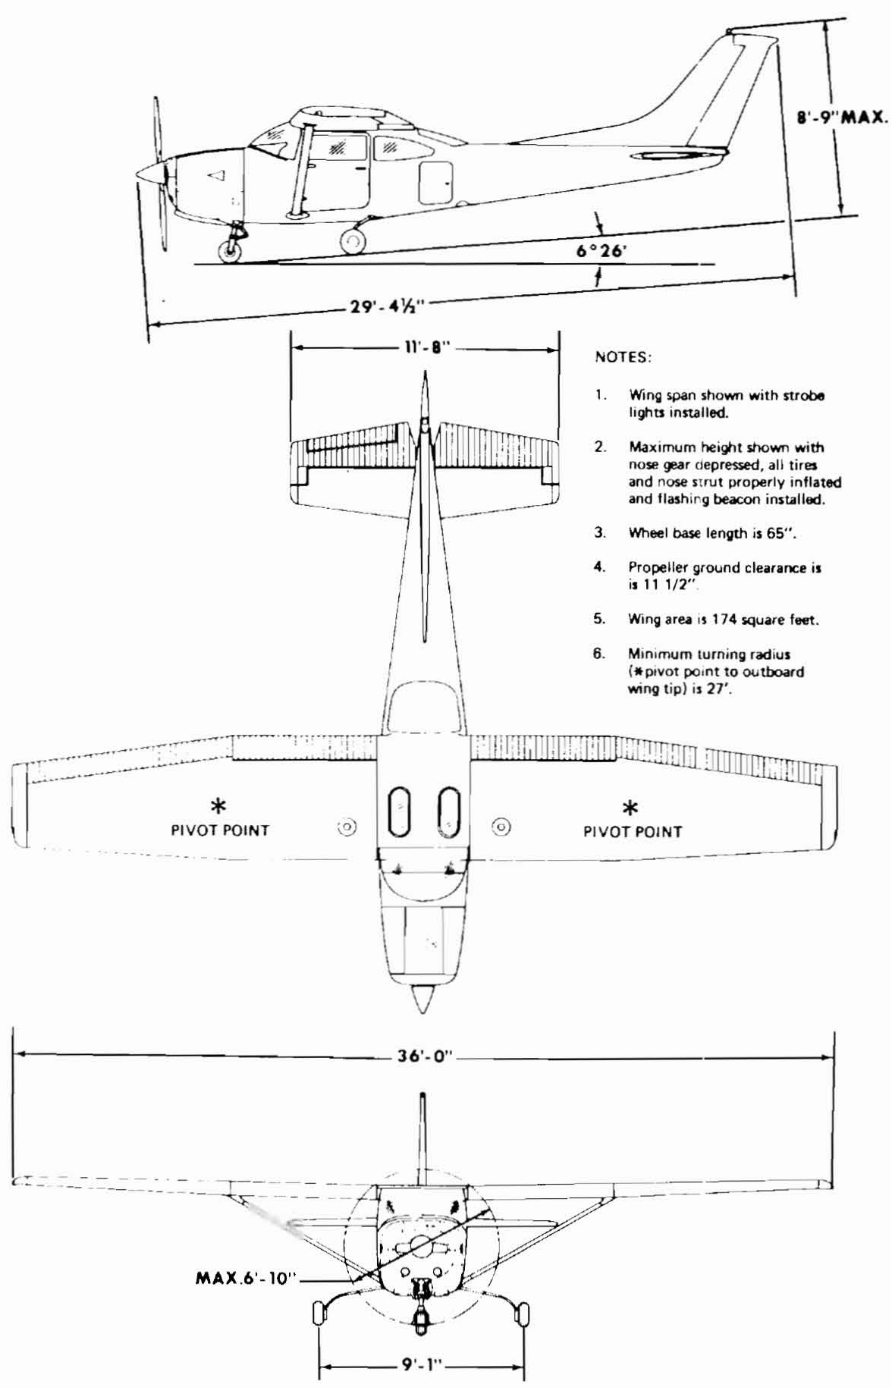
\includegraphics[width = 0.6\textwidth]{Technical Drawing/ThreeView.png}
    \caption{Three-view Drawing of Aircraft \footcite{POH}}
    \label{fig:threeview}
\end{figure}


\section{Methodology}

Using the three-view drawing from the POH, geometry of the aircraft can be measured with ImageJ, a free image manipulation program. A reference scale can be set using known distances on the drawings. Planform areas of the wing and empennage, the spans of the wing and empennage, and other various measurements can then be made with a reasonable degree of accuracy, with the assumption that the drawings are to scale. The aircraft is assumed to use a NACA 2412 cambered airfoil for the wing, and a NACA 0012 symmetric airfoil for the empennage.\\

\subsection{Wing}

\subsubsection{Zero Lift Drag}
Drag from the wing can be divided into two main components: base drag \cdo\ and lift-induced drag \cdi\. \cdo\ can be determined from aircraft geometry and flight conditions using the following equation\footcite{roskam}:
    
\begin{equation}
    C_{D_{0_w}} = R_{wf}R_{LS}C_f (1 + L^{'} (\frac{t}{c}) + 100 (\frac{t}{c})^4) \frac{S_{wet}}{S}
\end{equation}\\

\noindent Wing-fuselage interference factor $R_{wf}$ can be found from Figure 5.12 in the referenced document, from the fuselage Reynold's number $R_{N_f}$, which is found with:

\begin{equation}
    R_{N_f} = \frac{\rho V_\infty l_f}{\mu}
\end{equation}

\noindent Sweep dependent lift-correction factor $R_{LS}$ can similarly be referenced from Figure 5.12, as a function of sweep angle. As all lifting surfaces in the \plane\ have a sweep angle of $0$, $R_{LS}$ is identical for all components when required.\\

\noindent Airfoil thickness location parameter $L^{'}$ is a value dependent on the location of maximum thickness of the airfoil, and as the NACA 2412 has a maximum thickness located forward of the $\frac{1}{3}c$ location, the value of $L^{'}$ is 1.2 \footcite{roskam}.\\

\noindent Friction coefficient for flat plate equivalent $C_f$ is found using the following equation \footcite{roskam}:

\begin{equation}\label{eq:basedrag}
    C_f = \frac{0.455}{(\log_{10}(R_{N_w})^{2.58} (1 + 0.144 M^2)^{0.58}}
\end{equation}

\noindent where:

\begin{equation}
    R_{N_f} = \frac{\rho V_\infty \Bar{c}_w}{\mu_\infty}
\end{equation}

\\

Planform area of the wing $S$ is simple to find, and is measured using the three-view drawing in \ref{fig:threeview}. To find the wetted area of the wing $S_{wet}$, the following equation is used\footcite{toren}:


\begin{equation}
    S_{wet} = 2 \, S \,(1 + 0.25 (t/c)_r \frac{1 + \tau \lambda}{1 + \lambda})
\end{equation}

\noindent where:

\begin{equation*}
    \lambda = \frac{c_t}{c_r}
\end{equation*}

\noindent and:

\begin{equation*}
    \tau = \frac{(t/c)_t}{(t/c)_r}
\end{equation*}

\noindent The wing is broken into 3 component sections, and $S_{wet}$ of each is calculated individually. The first is the section of the wing with constant chord length, and runs between the edge of the canopy and the point at which the wing begins to taper. The second is the tapered section of the wing, which runs from the end of the constant chord section, and terminates at the wingtip. The final section is the section at which the wing mounts to the fuselage, over the canopy. It does not use the previous equation, and instead is simply summed as the planform area.\\

\subsubsection{Induced Drag}

Induced drag \cdi\ from the wing is drag created by the normal force component on the airfoil. It can be approximated using the following equation:

\begin{equation}
    C_{D_i} = \frac{C_L^2}{\pi e \AR}
\end{equation}

Assuming level flight, under pre-determined flight conditions (cruise at sea level, see \ref{app}), $C_L$ can be calculated from a given aircraft weight (see \ref{app}), and then used to find \cdi.

\subsection{Empennage}

The \cdo\ for both the vertical and horizontal components of the empennage are found using the same method used to find \cdo\ for the main wing. Planform area and span are measured using \ref{fig:threeview}, and $R_{wf}$ is reused, as its value is a function of fuselage geometry. $S_{wet}$ of the horizontal tail is calculated as a single, tapered section, and the vertical tail is calculated as two sections, as the taper angle of the vertical tail has a large variance near the base of the stabilizer. $C_f$ is then calculated using the respective $R_N_w$ for each component, and \cdo\ can be calculated using equation \ref{eq:basedrag}.\\

\subsection{Fuselage}

% Fuselage Geometry Measurement Explanation




\subsubsection{•}

\subsection{Required Engine Power}

\section{Results}
 

\section{Discussion}
 

\section{Conclusion}
 

\newpage
\section{References}

\printbibliography

\section{Appendix} \label{app}
\end{document}